\subsection{Linear Programming Modeling}

Consider the following problem statement. 

Two Crude Petroleum (TCP) runs a small refinery on the Texas coast.
The refinery distills crude petroleum from two sources, Country A and
Country B, into three main products: gasoline, jet fuel, and lubricants.
The two crudes differ in chemical composition and thus yield different
product mixes. Each barrel of Country A crude yields 0.3 barrel of
gasoline, 0.4 barrel of jet fuel, 0.2 barrel of lubricants, and 0.1 barrel of
waste. On the other hand, each barrel of Country B crude yields 0.4
barrel of gasoline, 0.2 barrel of jet fuel, 0.3 barrel of lubricants, and 0.1
barrel of waste. The crudes also differ in cost and availability. TCP can
purchase up to 9000 barrels per day from Country A at \$20 per barrel.
Up to 6000 barrels per day of Country B petroleum are also available
at the lower cost of \$15 per barrel because of the shorter
transportation distance. TCP's contracts with independent distributors
require it to produce 2000 barrels per day of gasoline, 1500 barrels per
day of jet fuel, and 500 barrels per day of lubricants. How can these
requirements be met most cost effectively?

Given the problem, we must now model it mathematically to solve. There 
are three components of a model: the \emph{decision variables}, the 
\emph{objective function}, and the \emph{constraints}. 

\paragraph{Decision variables}
In this example the only decision variables are the quantity of 
barrels to purchase from Country A, $x_1$, and from Country B, $x_2$. 

\paragraph{Objective function}
Minimize daily cost. 

\paragraph{Constraints}
\begin{itemize}
    \item Gasoline requirement
    \item Jet fuel requirement
    \item Lubricant requirement
    \item Country A availability
    \item Country B availability
    \item We must purchase natural numbers of barrels, not negative barrels, not fractional barrels, not imaginary numbers of barrels. 
    However, for the purposes of this problem, let us impose the weaker constraint of non-negativity.
\end{itemize}

Expressed mathematically, if $x_1$ is the amount of 
Country A crude refined per day in $10^3$ barrels and 
$x_2$ is amount of Country B crude refined per day in 
$10^3$ barrels, minimize the daily cost 
$\gamma = 20x_1 + 15x_2$ subject to the constraints:
\begin{align}
    0.3x_1 + 0.4x_2 &\geq 2 \\
    0.4x_1 + 0.2x_2 &\geq 1.5 \\
    0.2x_1 + 0.3x_2 &\geq 0.5 \\
    x_1 &\leq 9 \\
    x_2 &\leq 6 \\
    x_1, x_2 &\geq 0 
\end{align}
Note that that we may produce more than 
the demand; while this is suboptimal, if 
we set these constraints as equalities we may 
have a system of three equations 
with two unknowns and thus overconstraint 
ourselves and not be able to find a solution. 
    
This is the \emph{compact form} of the model, which 
we may now use an algorithm to solve. 
In this case, we can use the graphical method, 
which works if you have exactly two 
decision variables. First, 
we identify the feasible region.
\begin{enumerate}
    \item Plot all constraint lines at equality
    \item Determine the feasible sides of the constraint lines
    \item The feasible region must satisfy all constraints
\end{enumerate}
Next, find the improving 
direction of the objective 
function. 
\begin{enumerate}
    \item Arbitrarily plot two objective function lines
    \item Find the direction of improvement
\end{enumerate}
Finally, eyeball the optimal solution.
\begin{enumerate}
    \item Focus on corners of the feasible solution region
    \item Compute the numerical value from two crossing constraint lines
    \item There may be multiple optimal solutions
\end{enumerate}

\begin{figure}[ht]
\centering
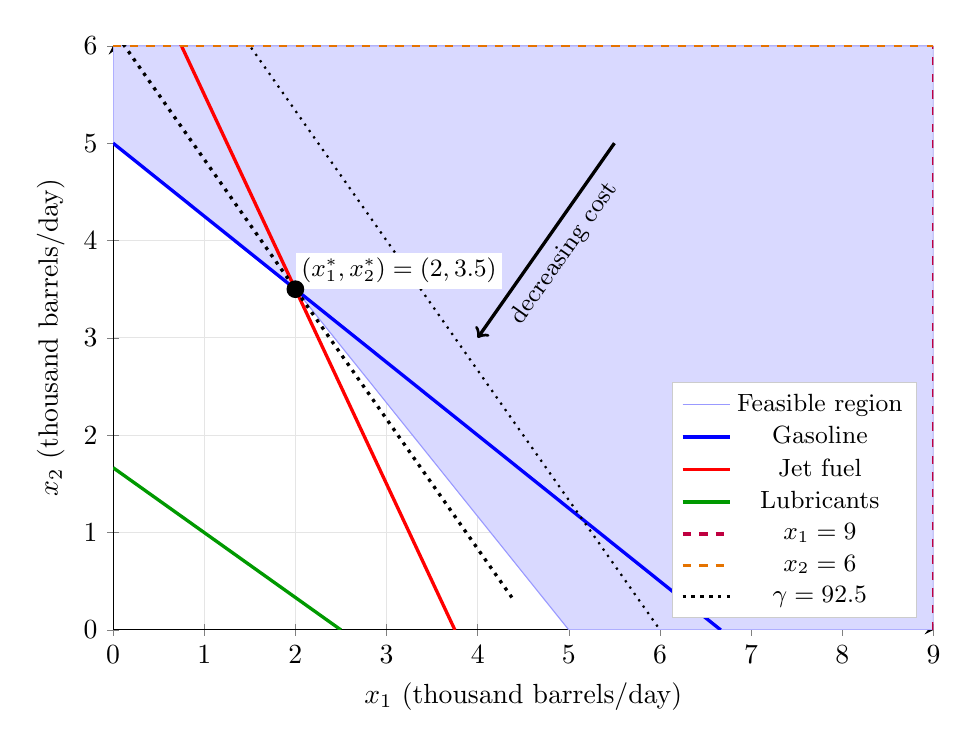
\begin{tikzpicture}
\begin{axis}[
    width=12cm,
    height=9cm,
    xmin=0, xmax=9,
    ymin=0, ymax=6,
    axis lines=left,
    xlabel={$x_1$ (thousand barrels/day)},
    ylabel={$x_2$ (thousand barrels/day)},
    grid=major,
    grid style={gray!20},
    legend style={
        at={(0.98,0.02)},
        anchor=south east,
        font=\small,
        fill=white,
        draw=gray!40
    },
]

% Feasible region
\addplot[
    fill=blue!15,
    draw=blue!40,
] coordinates {
    (0,6)
    (9,6)
    (9,0)
    (5,0)
    (2,3.5)
    (0,5)
    (0,6)
};
\addlegendentry{Feasible region}

% Gasoline constraint
% 0.3x_1 + 0.4x_2 = 2
% x_2 = 5 - 0.75x_1
\addplot[
    very thick,
    blue,
    domain=0:6.6667,
] {5 - 0.75*x};
\addlegendentry{Gasoline}

% Jet fuel constraint
% 0.4x_1 + 0.2x_2 = 1.5
% x_2 = 7.5 - 2x_1
\addplot[
    very thick,
    red,
    domain=0:3.75,
] {7.5 - 2*x};
\addlegendentry{Jet fuel}

% Lubricant constraint
% 0.2x_1 + 0.3x_2 = 0.5
% x_2 = 5/3 - 2/3 x_1
\addplot[
    very thick,
    green!60!black,
    domain=0:2.5,
] {5/3 - 2/3*x};
\addlegendentry{Lubricants}

% Country A availability
\addplot[
    very thick,
    purple,
    dashed,
] coordinates {(9,0) (9,6)};
\addlegendentry{$x_1=9$}

% Country B availability
\addplot[
    very thick,
    orange!90!black,
    dashed,
] coordinates {(0,6) (9,6)};
\addlegendentry{$x_2=6$}

% Objective contour: gamma = 92.5
% 20x_1 + 15x_2 = 92.5
% x_2 = 92.5/15 - 4/3 x_1
\addplot[
    very thick,
    black,
    dotted,
    domain=0:4.375,
] {92.5/15 - 4/3*x};
\addlegendentry{$\gamma=92.5$}

% Another objective contour
% gamma = 120
\addplot[
    thick,
    black,
    dotted,
    domain=0:6,
] {8 - 4/3*x};

% Optimal point
\addplot[
    only marks,
    mark=*,
    mark size=3pt,
    black,
] coordinates {(2,3.5)};

\node[
    anchor=south west,
    fill=white,
    inner sep=2pt,
    font=\small
] at (axis cs:2,3.5)
{$(x_1^*,x_2^*)=(2,3.5)$};

% Cost direction
\draw[
    ->,
    very thick,
] (axis cs:5.5,5)
    -- (axis cs:4,3)
    node[midway,below,sloped,font=\small]
    {decreasing cost};

\end{axis}
\end{tikzpicture}
\caption{TCP graph}
\label{fig:tcp-lp}
\end{figure}